\documentclass[]{book}
\usepackage{lmodern}
\usepackage{amssymb,amsmath}
\usepackage{ifxetex,ifluatex}
\usepackage{fixltx2e} % provides \textsubscript
\ifnum 0\ifxetex 1\fi\ifluatex 1\fi=0 % if pdftex
  \usepackage[T1]{fontenc}
  \usepackage[utf8]{inputenc}
\else % if luatex or xelatex
  \ifxetex
    \usepackage{mathspec}
    \usepackage{xltxtra,xunicode}
  \else
    \usepackage{fontspec}
  \fi
  \defaultfontfeatures{Mapping=tex-text,Scale=MatchLowercase}
  \newcommand{\euro}{€}
\fi
% use upquote if available, for straight quotes in verbatim environments
\IfFileExists{upquote.sty}{\usepackage{upquote}}{}
% use microtype if available
\IfFileExists{microtype.sty}{%
\usepackage{microtype}
\UseMicrotypeSet[protrusion]{basicmath} % disable protrusion for tt fonts
}{}
\usepackage{natbib}
\bibliographystyle{apalike}
\usepackage{color}
\usepackage{fancyvrb}
\newcommand{\VerbBar}{|}
\newcommand{\VERB}{\Verb[commandchars=\\\{\}]}
\DefineVerbatimEnvironment{Highlighting}{Verbatim}{commandchars=\\\{\}}
% Add ',fontsize=\small' for more characters per line
\usepackage{framed}
\definecolor{shadecolor}{RGB}{248,248,248}
\newenvironment{Shaded}{\begin{snugshade}}{\end{snugshade}}
\newcommand{\KeywordTok}[1]{\textcolor[rgb]{0.13,0.29,0.53}{\textbf{{#1}}}}
\newcommand{\DataTypeTok}[1]{\textcolor[rgb]{0.13,0.29,0.53}{{#1}}}
\newcommand{\DecValTok}[1]{\textcolor[rgb]{0.00,0.00,0.81}{{#1}}}
\newcommand{\BaseNTok}[1]{\textcolor[rgb]{0.00,0.00,0.81}{{#1}}}
\newcommand{\FloatTok}[1]{\textcolor[rgb]{0.00,0.00,0.81}{{#1}}}
\newcommand{\CharTok}[1]{\textcolor[rgb]{0.31,0.60,0.02}{{#1}}}
\newcommand{\StringTok}[1]{\textcolor[rgb]{0.31,0.60,0.02}{{#1}}}
\newcommand{\CommentTok}[1]{\textcolor[rgb]{0.56,0.35,0.01}{\textit{{#1}}}}
\newcommand{\OtherTok}[1]{\textcolor[rgb]{0.56,0.35,0.01}{{#1}}}
\newcommand{\AlertTok}[1]{\textcolor[rgb]{0.94,0.16,0.16}{{#1}}}
\newcommand{\FunctionTok}[1]{\textcolor[rgb]{0.00,0.00,0.00}{{#1}}}
\newcommand{\RegionMarkerTok}[1]{{#1}}
\newcommand{\ErrorTok}[1]{\textbf{{#1}}}
\newcommand{\NormalTok}[1]{{#1}}
\usepackage{longtable,booktabs}
\usepackage{graphicx}
\makeatletter
\def\maxwidth{\ifdim\Gin@nat@width>\linewidth\linewidth\else\Gin@nat@width\fi}
\def\maxheight{\ifdim\Gin@nat@height>\textheight\textheight\else\Gin@nat@height\fi}
\makeatother
% Scale images if necessary, so that they will not overflow the page
% margins by default, and it is still possible to overwrite the defaults
% using explicit options in \includegraphics[width, height, ...]{}
\setkeys{Gin}{width=\maxwidth,height=\maxheight,keepaspectratio}
\ifxetex
  \usepackage[setpagesize=false, % page size defined by xetex
              unicode=false, % unicode breaks when used with xetex
              xetex]{hyperref}
\else
  \usepackage[unicode=true]{hyperref}
\fi
\hypersetup{breaklinks=true,
            bookmarks=true,
            pdfauthor={Tyler Ransom},
            pdftitle={Advanced Structural Modeling},
            colorlinks=true,
            citecolor=blue,
            urlcolor=blue,
            linkcolor=magenta,
            pdfborder={0 0 0}}
\urlstyle{same}  % don't use monospace font for urls
\setlength{\parindent}{0pt}
\setlength{\parskip}{6pt plus 2pt minus 1pt}
\setlength{\emergencystretch}{3em}  % prevent overfull lines
\setcounter{secnumdepth}{5}

%%% Use protect on footnotes to avoid problems with footnotes in titles
\let\rmarkdownfootnote\footnote%
\def\footnote{\protect\rmarkdownfootnote}

%%% Change title format to be more compact
\usepackage{titling}

% Create subtitle command for use in maketitle
\providecommand{\subtitle}[1]{
  \posttitle{
    \begin{center}\large#1\end{center}
    }
}

\setlength{\droptitle}{-2em}

  \title{Advanced Structural Modeling}
    \pretitle{\vspace{\droptitle}\centering\huge}
  \posttitle{\par}
    \author{Tyler Ransom}
    \preauthor{\centering\large\emph}
  \postauthor{\par}
      \predate{\centering\large\emph}
  \postdate{\par}
    \date{2020-02-03}

\usepackage{booktabs}
\usepackage{amsthm}
\makeatletter
\def\thm@space@setup{%
  \thm@preskip=8pt plus 2pt minus 4pt
  \thm@postskip=\thm@preskip
}
\makeatother

\begin{document}

\maketitle


{
\hypersetup{linkcolor=black}
\setcounter{tocdepth}{2}
\tableofcontents
}
\section{Prerequisites}\label{prerequisites}

You should know everything in PhD Econometrics I and Econometrics II
before taking this class.

\section{What is Structural Modeling?}\label{intro}

In this chapter, I explain what structural modeling is and how it can be
useful to economists. A nice treatment of this topic is
\citet{reissWolak2007}, which I borrow some materials from.

In the simplest sense, structural modeling (or, interchangeably,
structural econometrics) is a combination of economic and statistical
models. Structural models are used in every empirical field of
economics: from dynamic stochastic general equilibrium (DSGE) models in
macroeconomics to models of firm decision-making in industrial
organization to individual choice models in labor.

More formally, a structural model is an attempt to estimate
\textbf{policy-invariant fundamental parameters}, also known as
structural parameters. The parameter estimates can then be used to
predict outcomes in a counterfactual setting. Typically, structural
parameters are those parameters which enter an agent's utility function
or production function (and cost function). Structural models may also
incorporate constraints faced by the agent(s), strategic behavior among
competing agents, or other aspects of economic theory such as moral
hazard in a principal-agent scenario. Once the econometrician knows the
preferences, production technology, and constraints of the agent(s), she
can predict how the agent(s) will behave in a new scenario for which
there is no existing data.

Structural models are especially useful in settings where an experiment
cannot be undertaken. In this case, one must specify how the
unobservables are related to the observables, because this relationship
cannot be ignored without the randomization that occurs in an
experiment.

\subsection{Advantages and Disadvantages of Structural
Models}\label{advantages-and-disadvantages-of-structural-models}

Many economists shy away from structural models because using them
forces the researcher to make strong assumptions about how the world
works. In essence a structural model is a researcher's view of the
world. To the extent that the model includes unreasonable or unrealistic
assumptions, one must discount any results derived from the model.

Another reason some economists dislike structural models is because they
can be difficult to estimate. Structural models typically are nonlinear
(even if they are linear-in-parameters) and estimation typically
requires using maximum likelihood or method of moments estimation as
opposed to linear regression techniques.

The main advantage of using a structural model is that it can be a
powerful tool for predicting the effects of potential policies. If one
knows the data generating process (DGP), then one does not need to do
any statistical estimation. Structural modeling is an attempt to
estimate the parameters of the DGP. Once the DGP is known, one can use
it to simulate what might happen under counterfactual scenarios.

\subsection{A simple structural model}\label{a-simple-structural-model}

One toy example that often appears in introductory econometrics
textbooks is the effect of education on earnings. Typically, the
textbook presents an equation like this:
\[\log\left(wage_{i}\right)=\beta_0 + \beta_{1}educ_{i}+\varepsilon_{i}\]
where $wage_i$ is the individual's wage as an adult, and $educ_i$ is the
individual's years of completed education (e.g.~12 for a high school
graduate, 16 for a college graduate, etc.).

\subsection{Other examples}\label{other-examples}

\begin{itemize}
\itemsep1pt\parskip0pt\parsep0pt
\item
  Tuition subsidy (\citet{keaneWolpin1997})
\item
  IO demand estimation (BLP, etc.)
\item
  IO production function estimation (Collard-Wexler papers)
\item
  IO entry games (\ldots{})
\item
  Trade markups (\citet{deLoecker_al2018})
\item
  Development (\ldots{})
\item
  Migration (\citet{kennanWalker2011})
\item
  Regional demand and commuting flows (\citet{monte_al2018})
\end{itemize}

You can label chapter and section titles using \texttt{\{\#label\}}
after them, e.g., we can reference Chapter \ref{intro}. If you do not
manually label them, there will be automatic labels anyway, e.g.,
Chapter \ref{methods}.

Figures and tables with captions will be placed in \texttt{figure} and
\texttt{table} environments, respectively.

\begin{Shaded}
\begin{Highlighting}[]
\KeywordTok{par}\NormalTok{(}\DataTypeTok{mar =} \KeywordTok{c}\NormalTok{(}\DecValTok{4}\NormalTok{, }\DecValTok{4}\NormalTok{, .}\DecValTok{1}\NormalTok{, .}\DecValTok{1}\NormalTok{))}
\KeywordTok{plot}\NormalTok{(pressure, }\DataTypeTok{type =} \StringTok{'b'}\NormalTok{, }\DataTypeTok{pch =} \DecValTok{19}\NormalTok{)}
\end{Highlighting}
\end{Shaded}

\begin{figure}

{\centering 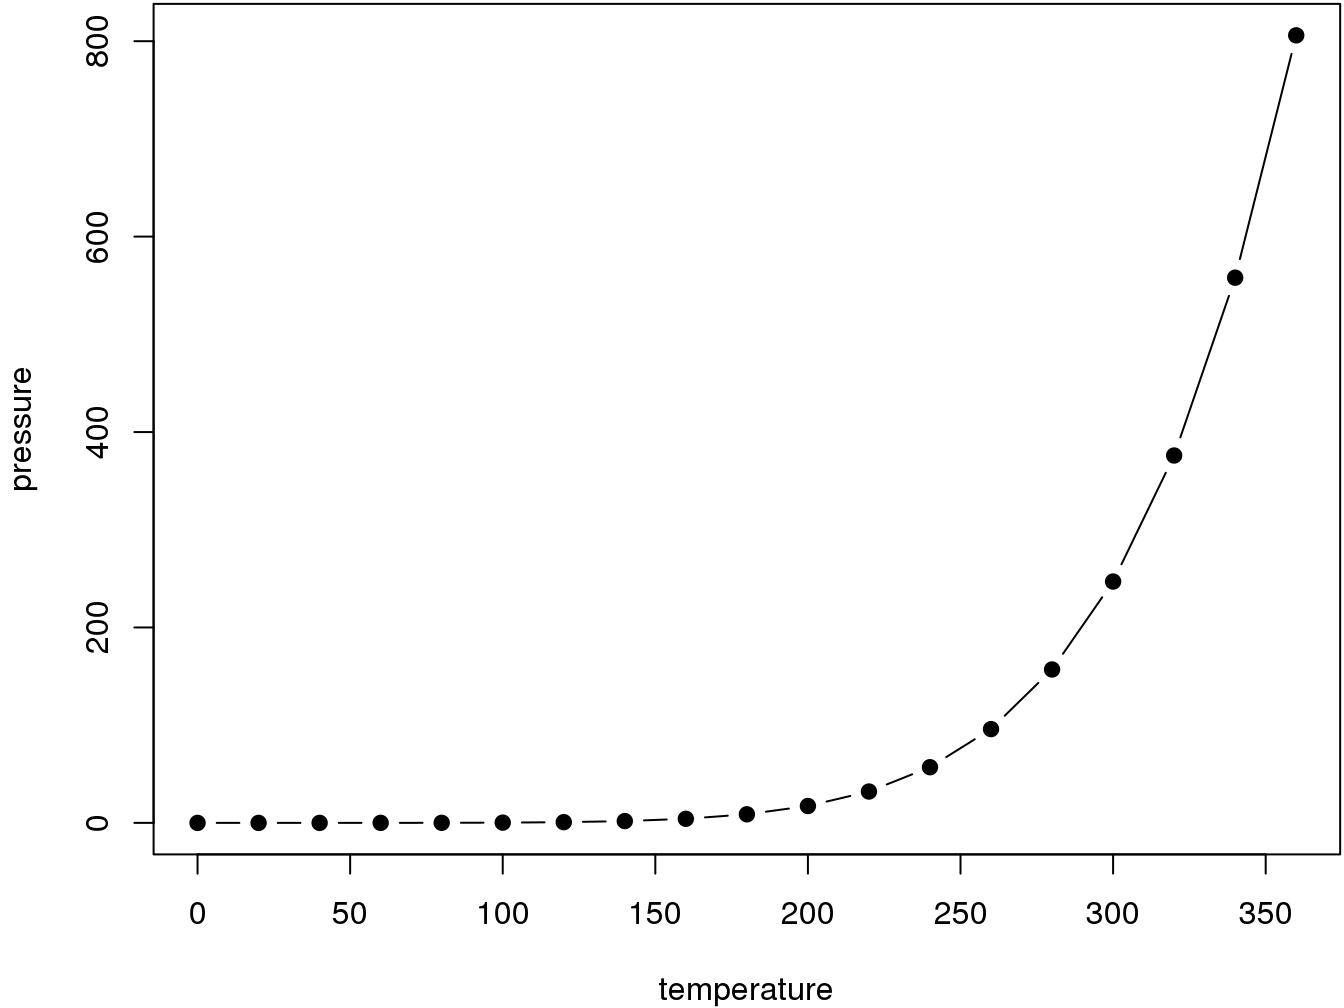
\includegraphics[width=0.8\linewidth]{PhDmetrics_files/figure-latex/nice-fig-1} 

}

\caption{Here is a nice figure!}\label{fig:nice-fig}
\end{figure}

Reference a figure by its code chunk label with the \texttt{fig:}
prefix, e.g., see Figure \ref{fig:nice-fig}. Similarly, you can
reference tables generated from \texttt{knitr::kable()}, e.g., see Table
\ref{tab:nice-tab}.

\begin{Shaded}
\begin{Highlighting}[]
\NormalTok{knitr::}\KeywordTok{kable}\NormalTok{(}
  \KeywordTok{head}\NormalTok{(iris, }\DecValTok{20}\NormalTok{), }\DataTypeTok{caption =} \StringTok{'Here is a nice table!'}\NormalTok{,}
  \DataTypeTok{booktabs =} \OtherTok{TRUE}
\NormalTok{)}
\end{Highlighting}
\end{Shaded}

\begin{table}[t]

\caption{\label{tab:nice-tab}Here is a nice table!}
\centering
\begin{tabular}{rrrrl}
\toprule
Sepal.Length & Sepal.Width & Petal.Length & Petal.Width & Species\\
\midrule
5.1 & 3.5 & 1.4 & 0.2 & setosa\\
4.9 & 3.0 & 1.4 & 0.2 & setosa\\
4.7 & 3.2 & 1.3 & 0.2 & setosa\\
4.6 & 3.1 & 1.5 & 0.2 & setosa\\
5.0 & 3.6 & 1.4 & 0.2 & setosa\\
\addlinespace
5.4 & 3.9 & 1.7 & 0.4 & setosa\\
4.6 & 3.4 & 1.4 & 0.3 & setosa\\
5.0 & 3.4 & 1.5 & 0.2 & setosa\\
4.4 & 2.9 & 1.4 & 0.2 & setosa\\
4.9 & 3.1 & 1.5 & 0.1 & setosa\\
\addlinespace
5.4 & 3.7 & 1.5 & 0.2 & setosa\\
4.8 & 3.4 & 1.6 & 0.2 & setosa\\
4.8 & 3.0 & 1.4 & 0.1 & setosa\\
4.3 & 3.0 & 1.1 & 0.1 & setosa\\
5.8 & 4.0 & 1.2 & 0.2 & setosa\\
\addlinespace
5.7 & 4.4 & 1.5 & 0.4 & setosa\\
5.4 & 3.9 & 1.3 & 0.4 & setosa\\
5.1 & 3.5 & 1.4 & 0.3 & setosa\\
5.7 & 3.8 & 1.7 & 0.3 & setosa\\
5.1 & 3.8 & 1.5 & 0.3 & setosa\\
\bottomrule
\end{tabular}
\end{table}

\section{Static Discrete Choice
Models}\label{static-discrete-choice-models}

\subsection{In this chapter}\label{in-this-chapter}

\begin{enumerate}
\def\labelenumi{\arabic{enumi}.}
\item
  Describe static discrete choice models
\item
  Derive logit probabilities
\item
  Show how to estimate logits and multinomial logits
\item
  Cover the IIA property
\item
  Discuss expected utility and consumer surplus
\end{enumerate}

\subsection{Notation}\label{notation}

Let $d_i$ indicate the choice individual $i$ makes where
$d_i\in\{1,\cdots, J\}$. Individuals choose $d$ to maximize their
utility, $U$. $U$ generally is written as:
\[U_{ij}=u_{ij}+\varepsilon_{ij}\] where:

\begin{enumerate}
\def\labelenumi{\arabic{enumi}.}
\item
  $u_{ij}$ relates observed factors to the utility individual $i$
  receives from choosing option $j$
\item
  $\varepsilon_{ij}$ are unobserved to the econometrician but observed
  to the individual
\item
  $d_{ij}=1$ if $u_{ij}+\varepsilon_{ij}>u_{ij'}+\varepsilon_{ij'}$ for
  all $j'\neq j$
\end{enumerate}

\subsection{Probabilities}\label{probabilities}

With the $\varepsilon$'s unobserved, the probability of individual $i$
making choice $j$ is given by: \[\begin{aligned}
P_{ij}&=\Pr(u_{ij}+\varepsilon_{ij}>u_{ij'}+\varepsilon_{ij'}\forall j'\neq j)\\
&=\Pr(\varepsilon_{ij'}-\varepsilon_{ij}<u_{ij}-u_{ij'}\forall j'\neq j)\\
&=\int_{\varepsilon}I(\varepsilon_{ij'}-\varepsilon_{ij}<u_{ij}-u_{ij'}\forall j'\neq j)f(\varepsilon)d\varepsilon\end{aligned}\]
Note that, regardless of what distributional assumptions are made on the
$\varepsilon$'s, the probability of choosing a particular option does
not change when we:

\begin{enumerate}
\def\labelenumi{\arabic{enumi}.}
\item
  Add a constant to the utility of all options (utility is relative to
  one of the options, only differences in utility matter)
\item
  Multiply by a positive number (need to scale something, generally the
  variance of the $\varepsilon$'s)
\end{enumerate}

\subsection{Variables}\label{variables}

Suppose we have: \[\begin{aligned}
u_{i1}&=\alpha Male_i+\beta_1 X_i + \gamma Z_1\\
u_{i2}&=\alpha Male_i+\beta_2 X_i+\gamma Z_2\end{aligned}\] Since only
differences in utility matter:
\[u_{i1}-u_{i2}=(\beta_1-\beta_2)X_i+\gamma (Z_1-Z_2)\] Thus, we cannot
tell whether men are happier than women, but can tell whether men have a
preference for a particular option over another. We can only obtain
differenced coefficient estimates on $X$'s, and can obtain an estimate
of a coefficient that is constant across choices only if the variable it
is hitting varies by choice.

\section{Methods}\label{methods}

We describe our methods in this chapter.

\section{Applications}\label{applications}

Some \emph{significant} applications are demonstrated in this chapter.

\subsection{Example one}\label{example-one}

\subsection{Example two}\label{example-two}

\section{Final Words}\label{final-words}

We have finished a nice book.

\end{document}
